\section{Background}
\label{sec:background}

We begin with some background on quantum computing and quantum algorithms. 

\noindent\textbf{\textit{Quantum States.}} A quantum state consists of one or more quantum bits (\emph{qubits}). A qubit can be expressed as a two dimensional vector $\begin{psmallmatrix} \alpha \\ \beta \end{psmallmatrix}$ where $\alpha,\beta$ are complex numbers such that $|\alpha|^2 + |\beta|^2 = 1$.  The $\alpha$ and $\beta$ are called \emph{amplitudes}. 
%
We frequently write the qubit vector as $\alpha\ket{0} + \beta\ket{1}$ where $\ket{0} = \begin{psmallmatrix} 1 \\ 0 \end{psmallmatrix}$ and $\ket{1} = \begin{psmallmatrix} 0 \\ 1 \end{psmallmatrix}$ are \emph{computational basis states}. When both $\alpha$ and $\beta$ are non-zero, we can think of the qubit as being ``both 0 and 1 at once,'' a.k.a. a \emph{superposition}. For example, $\frac{1}{\sqrt{2}}(\ket{0} + \ket{1})$ is an equal superposition of $\ket{0}$ and $\ket{1}$. 

We can join multiple qubits together to form a larger quantum state with the \emph{tensor product} ($\otimes$) from linear algebra. For example, the two-qubit state $\ket{0} \otimes \ket{1}$ (also written as $\ket{01}$) corresponds to vector $[~0~1~0~0~]^T$. 
Sometimes a multi-qubit state cannot be expressed as the tensor of individual states; such states are called \emph{entangled}. One example is the state $\frac{1}{\sqrt{2}}(\ket{00} + \ket{11})$, known as a \emph{Bell pair}.
Entangled states lead to exponential blowup: A general $n$-qubit state must be described with a $2^n$-length vector, rather than $n$ vectors of length two.

\begin{figure}[t]
{\centering
\hspace*{-1em}
          \begin{minipage}[b]{.20\textwidth}
            {\qquad
              \footnotesize
              \Qcircuit @C=0.5em @R=0.5em {
                \lstick{\ket{0}} & \gate{H} & \ctrl{1} & \qw &\qw & & \dots & \\
                \lstick{\ket{0}} & \qw & \targ & \ctrl{1} & \qw & &  \dots &  \\
                \lstick{\ket{0}} & \qw & \qw   & \targ & \qw & &  \dots &  \\
                & \vdots &   &  &  & & & \\
                & \vdots &  & \dots & & & \ctrl{1} & \qw  \\
                \lstick{\ket{0}} & \qw & \qw & \qw &\qw &\qw & \targ & \qw
              }
            }
\caption{GHZ}
\label{fig:circuit-example}
\end{minipage}
\hfill
\begin{minipage}[b]{.40\textwidth}
                 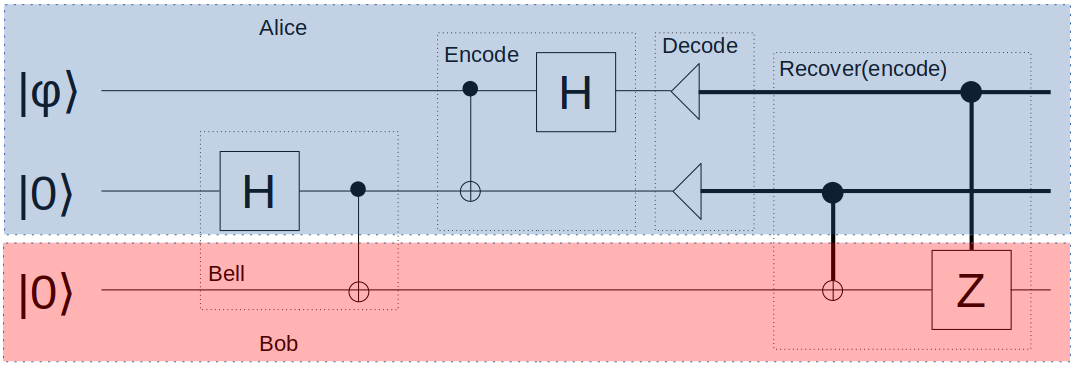
\includegraphics[width=1\textwidth]{tele_circuit.png}
            \caption{Teleportation Circuit}
            \label{fig:background-circuit-examplea}
 \end{minipage}
\hfill
\begin{minipage}[b]{.39\textwidth}
                 \includegraphics[width=1\textwidth]{swaps.png}
            \caption{Quantum Routing}
            \label{fig:background-circuit-exampleb}
          \end{minipage}
}
\end{figure}

\noindent\textbf{\textit{Quantum Computations and the First Quantum Abstraction.}} High-level quantum programming languages are usually designed to follow the \emph{QRAM model}~\cite{Knill1996}, where quantum computers are used as co-processors to classical computers. The classical computer generates descriptions of circuits to send to the quantum computer and then processes the measurement results.
Computation on a quantum value state consists of a series of \emph{quantum operations}, each of which acts on a subset of qubits in the value state. 
In the standard presentation, quantum computations are expressed as \emph{circuits}, as shown in \Cref{fig:circuit-example},
which takes a qubit array and constructs a circuit that prepares the Greenberger-Horne-Zeilinger (GHZ) state \cite{Greenberger1989}, which is an $n$-qubit entangled quantum state of the form
{
\begin{center}
$
    \ket{\text{GHZ}^n} = \frac{1}{\sqrt{2}}(\ket{0}^{\otimes n}+\ket{1}^{\otimes n}).
$
\end{center}
}
In these circuits, each horizontal wire represents a qubit and boxes on these wires indicate quantum operations, or \emph{gates}. 
Applying a gate to a state \emph{evolves} the state. The traditional semantics of doing so is expressed by multiplying the state vector by the gate's corresponding matrix representation; single-qubit gates are 2-by-2 matrices, and two-qubit gates are 4-by-4 matrices. A gate's matrix must be \emph{unitary}, ensuring that it preserves the unitarity invariant of quantum states' amplitudes. An entire circuit can be expressed as a matrix by composing its constituent gates.
The GHZ circuit applies a \emph{Hadamard} (\coqe{H}) to turn the first qubit into superposition. The very next \emph{controlled-not} (\coqe{CNOT}) gate application entangles the second qubit with the superposition qubit; thus, creates a Bell pair.
Each of the next series of \emph{controlled-not} (\coqe{CNOT}) gate applications transitively moves one qubit to join the entanglement cluster and finally creates the $\ket{\text{GHZ}^n}$ state above. Essentially, a $\ket{\text{GHZ}^n}$ state is a generalized version of Bell pairs.

A \emph{measurement} operation extracts classical information from a quantum state, typically when a computation completes. Measurement collapses the state to a basis states with a probability related to the state's amplitudes. For example, measuring $\frac{1}{\sqrt{2}}(\ket{0} + \ket{1})$ in the computational basis will collapse the state to $\ket{0}$ with probability $\frac{1}{2}$ and likewise for $\ket{1}$, returning classical value $0$ or $1$, respectively.
The circuit representations are typically expressed as the \coqe{meas} gates in \Cref{fig:background-circuit-examplea}.

The above examples indicate that most current quantum programming languages tend to focus on the circuit level physical details of quantum computation behaviors rather than providing high level abstractions \cite{VOQC}.
For abstracting away circuit details but keeping the essence of quantum behaviors,
one really needs to focus on the utilities of different small quantum algorithms, such as GHZ,
because quantum computations for solving a task are typically constructed based on a limited set of small algorithms.
For quantum network communications, the essence of GHZ provides a quantum channel to connect different parties.
If we view the $n$ different qubits in GHZ as $n$ different parties,
measuring any qubit resulting in a bit, either $0$ or $1$, makes other parties consensually produce the same bit.
Thus, the GHZ circuit can be thought abstractly as a channel to agree on all parties.
We will see two more small algorithm abstractions below.

\noindent\textbf{\textit{Quantum Teleportation For Network Communications and Abstraction.}}
Quantum teleportation \cite{PhysRevLett.70.1895,Rigolin_2005} is an algorithm to communicate a quantum message, a single qubit or multiple qubits, between two parties.
Almost all quantum network protocols are originated from the algorithm.
The circuit diagram in \Cref{fig:background-circuit-examplea} describes a quantum teleportation circuit for communicating a qubit message between Alice and Bob.
In the circuit in \Cref{fig:background-circuit-examplea},
Alice holds a quantum qubit message, represented as the first qubit line, and a $\ket{0}$ qubit;
while Bob holds the third $\ket{0}$ qubit.
The application \coqe{bel1000} creates a quantum channel (Bell pair) between Alice's second qubit and Bob's qubit.

The \coqe{alice} application in \Cref{fig:background-circuit-examplea} does two tasks: 1) it pushes Alice's qubit message $\varphi$ to attach to the quantum channel between Alice and Bob; and 2) Alice then measures her two qubits, which destroys the entangled three qubits and results in two classical bits held by Alice and one classical bit held by Bob.
The \coqe{bob} application also has two tasks: 1) it uses the bold classical message channel to send Alice's two classical bits to Bob; and 2) Bob receives the two classical bits and uses a proper devices, the \coqe{X} and \coqe{Z} gates, to recover the message $\varphi$, stored in Bob's qubit.

Regardless the circuit details, the quantum teleportation procedure can be summarized as five steps:
1) we create a quantum channel between Alice and Bob;
2) we push Alice's quantum message to the quantum channel;
3) Alice measures and destroys her two qubits, so Alice has two classical remains while Bob has one;
4) Alice sends Bob two classical bits;
and 5) Bob recovers the quantum message based on the three classical bits.

The multiple qubit version of quantum teleportation \cite{Rigolin_2005} is proportional to the single qubit version
and has the same procedure.
Since every quantum network protocol utilizes the algorithm, we model these five steps as five operations in QAM.

\noindent\textbf{\textit{Hybrid Quantum Classical Network with Quantum Routing.}}
There are two observations from quantum teleportation. First, the network protocol describes a hybrid quantum classical network because it combines quantum and classical channels to hand a quantum message from Alice to Bob. Handing here refers to the fact that once Bob receives the quantum message, Alice's copy is destroyed. Second, A long distance quantum channel can be built through the GHZ algorithm, since a Bell pair is essentially $2$-qubit GHZ.

Unfortunately, it is impossible to practically build a quantum channel through the $n$-party (more than $2$) GHZ algorithm across different machines \cite{Illiano_2022}, even though it is theatrically possible.
A typical quantum channel establishment is done through three steps: 1) a classical network communication process is applied to find a path from the source to the target of a message communication, such as Alice and Bob in \Cref{fig:background-circuit-exampleb}, respectively; 2) any two of nodes in the path are established a quantum channel by a Bell pair, such as the pair of Alice and the repeater, as well as the pair of the repeater and Bob in \Cref{fig:background-circuit-exampleb}; 3) a swap operation is applied to the two pairs and a quantum channel is then built from the source to the target, as the Alice and Bob pair in \Cref{fig:background-circuit-exampleb}(d).

Quantum teleportation describes the circuit details of communicating quantum messages through two parties.
For a long distance communication, the quantum routing concept is involved.
A typical and near term possible technique to send quantum information through long distance is \textit{entanglement swap},
which relies on intermediate quantum repeaters between the two parties. Suppose Alice and Bob stay in two separate places and there is a quantum repeater, $r_1$ between them, they can create a long-distance entanglement in two steps. First, Alice and Bob each create an entanglement state with $r_1$; then $r_1$ performs a Bell state measurement locally. After measurement, the two original entanglements are destroyed and therefore, a new entanglement pair is created between Alice and Bob. 

In this paper, we first establish a system to describe quantum teleportation with the GHZ quantum channel building algorithm;
we then upgrade the system to include the quantum routing algorithm, as well as establishing an evaluation system to allow users to build quantum network protocols and evaluate their performance.

\liyi{Le: need better description. Please help find the CHEM paper and modify. }
\noindent\textbf{\textit{Chemical Abstract Machine.}} Chemical abstract machine \cite{BERRY1992217} models multi-party communication behaviors as chemical reactions, where processes live in molecule membrane structures, named \textit{cells} in QAM, and they can react by the reaction rules defining how molecule membranes can connect together and processes living inside a membrane can also communicate through the heating and cooling rules, 
defining the transformation between process active and inactive states, where active and inactive states represent processes being able to communicate or not.

% Writing a quantum algorithm now, with SQIR (but likewise with Quipper, Pyquil, Circ, etc.). Example: Shor’s
% Write quantum parts (QPE) 
% Classical parts via library functions in meta-language (Modular multiplier)
% Refer to particular quipper functions, e.g., for adding, subtraction, etc.
% https://www.mathstat.dal.ca/~selinger/quipper/doc/Quipper-Libraries-QFTAdd.html qft_add_in_place :: QDInt -> QDInt -> Circ (QDInt, QDInt), Add one QDInt onto a second, in place; i.e. (x,y) ↦ (x,x+y). Arguments are assumed to be of equal size. This implementation follows the implementation in Thomas G. Draper's paper "Addition on a Quantum Computer" which doesn't require the use of any ancilla qubits through a clever use of the quantum Fourier transform.
% Mention Q# too
% https://github.com/microsoft/QuantumLibraries/tree/main/Numerics/src
% Maybe Scaffold:
% Write oracles via “RKQC intrinsic” functions (see sec 4.1 of https://iopscience.iop.org/article/10.1088/2058-9565/ab8c2c/pdf). The intrinsics they talk about here are super simple (swap two registers or add two registers together)
% Quipper: Write in Haskell, build_circuit, is better
% Problems to solve: Efficient compilation, verification of that compilation
% Verification: Prior work with ReverC, but only classical gates
